\section{Auswertung}
\label{sec:Auswertung}
\subsection{Bestimmung der Brennweite über Linsengleichung}
Die gemessenen Werte  der Gegenstandsweite $g$ und der Bildweite $b$  sind
in der Tabelle \ref{tab:1} und \ref{tab:2} aufgeliste.
Die Linse der ersten Messung besitzt laut Herstellerangaben eine Brennweite $f$
von
\begin{align*}
  f_1=100\si{\milli\meter}\\
\intertext{und die der zweiten Linse eine von }
  f_2=150\si{\milli\meter}.
\end{align*}
Die gemessene Gegenstandsweiten und Bildweiten können nun in die Gleichung
\eqref{eqn:linse} eingesetzet werden um die entsprechende Brennweite $f$
zu erhalen. Ebenfalls ist in der Tabelle \ref{tab:1}
die Bildgröße enthalten somit lässt sich durch die Gegenstandsgröße, die
\begin{align*}
  G=30\si{\milli\meter}
\end{align*}
beträt, das Verhältnis zwischen $G/B$ und $g/b$ vergleichen. Dies ist ebenfalls
in der Tabelle \ref{tab:1} aufgelistet.
\begin{table}
  \centering
  \caption{Messwerte der 1. Messung und das aus der Gleichung
   \eqref{eqn:linse} berechnete $f$.}
  \label{tab:1}
  \begin{tabular}{c c c c c c}
  \toprule
  Gegenstandsweite   & Bildweite & Bildgröße & Brennweite & \multicolumn{2}{c}{Verhältniss}\\
  $g/\si{\milli\meter}$ & $b/\si{\milli\meter}$ & $B/\si{\milli\meter}$& $f/\si{\milli\meter}$& $G/B$ &$g/b$\\
  \midrule
  140   &   317  &   60 & 97 &0,5 &0,4 \\
  150   &   284  &   47 & 98 &0,6 &0,5 \\
  160   &   251  &   43 & 98 &0,7 &0,6 \\
  200   &   168  &   27 & 91 &1,1 &1,2 \\
  230   &   170  &   20 & 98 &1,5 &1,4 \\
  250   &   158  &   18 & 97 &1,7 &1,6 \\
  280   &   150  &   16 & 98 &1,9 &1,9 \\
  300   &   123  &   16 & 87 &1,9 &2,4 \\
  320   &   140  &   14 & 97 &2,1 &2,3 \\
  350   &   134  &   12 & 97 &2,5 &2,6 \\
  \bottomrule
 \end{tabular}
\end{table}

\begin{table}
  \centering
  \caption{Messwerte der 2. Messung und das aus der Gleichung
   \eqref{eqn:linse} berechnete $f$.}
  \label{tab:2}
  \begin{tabular}{c c c}
  \toprule
  Gegenstandsweite   & Bildweite & Brennweite\\
  $g/\si{\milli\meter}$ & $b/\si{\milli\meter}$ & $f/\si{\milli\meter}$\\
  \midrule
  260  &  431 & 162\\
  250  &  480 & 164\\
  270  &  414 & 163\\
  280  &  395 & 164\\
  290  &  375 & 164\\
  300  &  357 & 163\\
  330  &  320 & 162\\
  350  &  306 & 163\\
  370  &  291 & 163\\
  400  &  275 & 163\\
  \bottomrule
\end{tabular}
\end{table}

Werden die berechnenten Brennweiten $f$
nun gemittelt, ergibt sich für die erste Linse:
\begin{align*}
  f_{1_\mathrm{gemessen}}=(95,8\pm3,4)\si{\milli\meter}
\intertext{Für die zweite Linse:}
f_{2_\mathrm{gemessen}}=(163,2\pm0,6)\si{\milli\meter}
\end{align*}

Desweitern lassen sich die Genauigkeiten der Messwerte überprüfen,
indem die gemessene Gegenstandsweiten $g$ auf die x-Achse aufgetragen wird
und mit den entsprechenden Bildweiten $b$, die auf der y-Achse aufgertagen ist,
durch eine Linie verbunden wird. Die Abbildungen \ref{fig:1} und \ref{fig:2}
enthälten diese Methode.

\begin{figure}
 \centering
 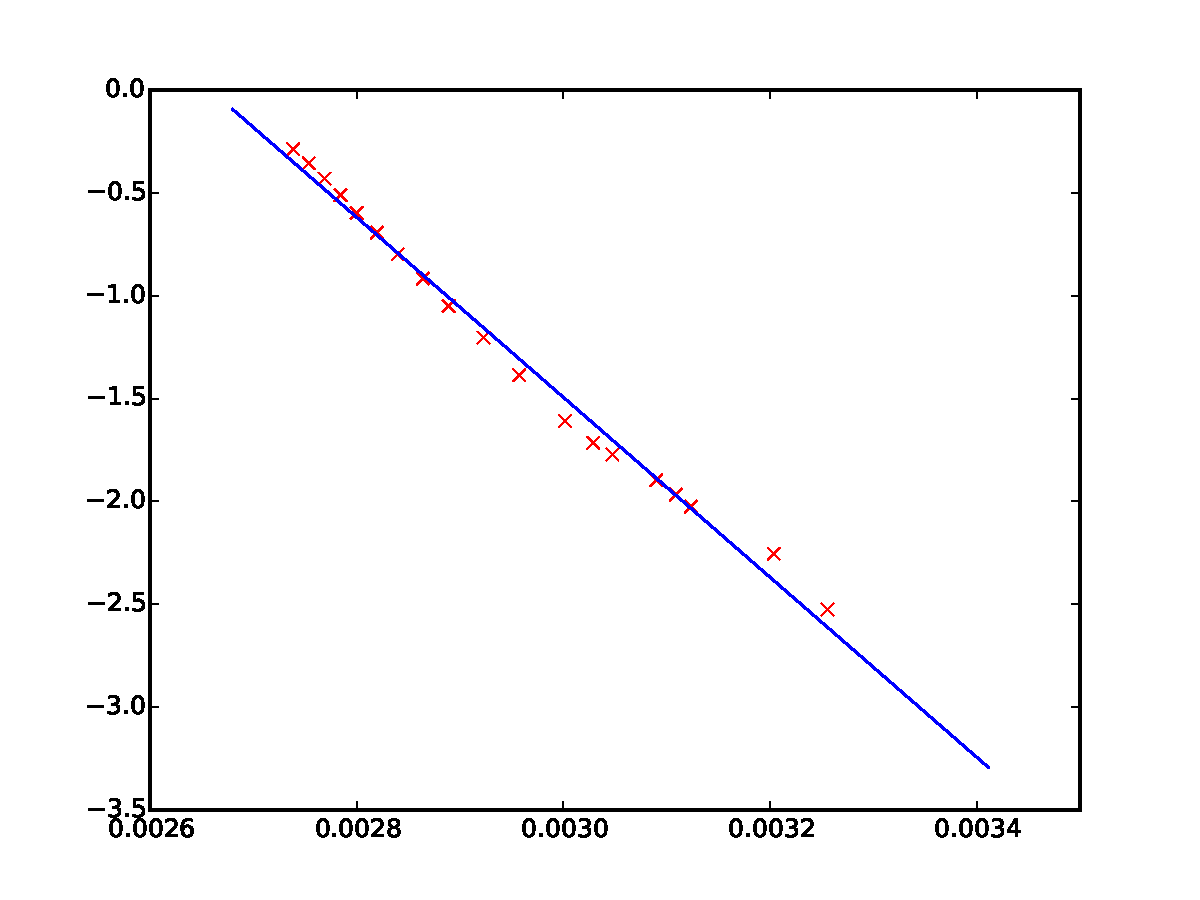
\includegraphics[width=0.7\textwidth]{plot1.pdf}
 \caption{Abblidung zur Bestimmung der Genauigkeit der 1. Messung}
 \label{fig:1}
\end{figure}

\begin{figure}
 \centering
 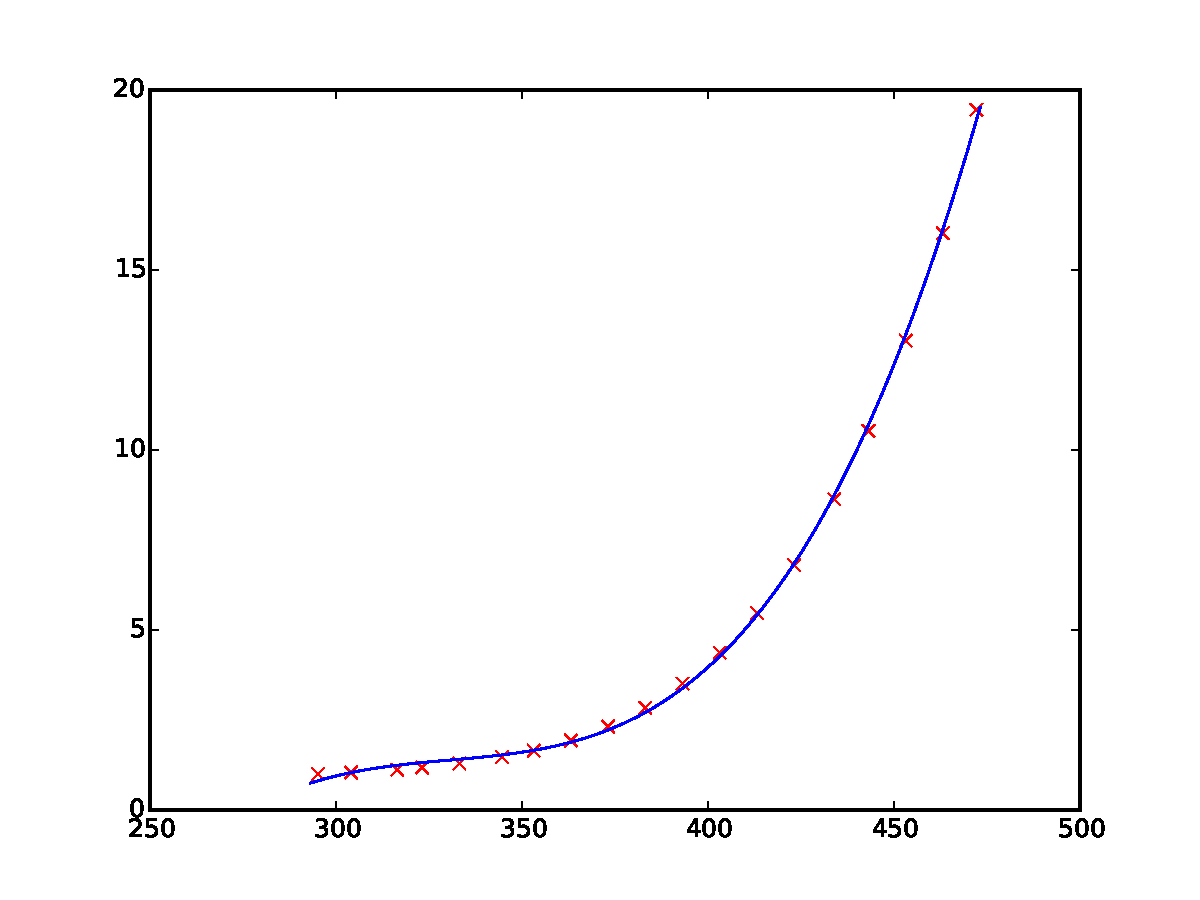
\includegraphics[width=0.7\textwidth]{plot2.pdf}
 \caption{Abblidung zur Bestimmung der Genauigkeit der 2. Messung}
 \label{fig:2}
\end{figure}

\subsection{Bestimmung der Brennweite durch die Methode von Bessel}

  \begin{table}
    \centering
    \caption{Messwerte die mit Hilfe der Methode von Bessel aufgenommen worden sind
    und die Brennweiten $f$ die über die Formel \eqref{eqn:Bessel} berechnet werden.}
    \label{tab:bessel}
    \begin{tabular}{c c c c c c c}
    \toprule
    Gegenstandsweite   & Bildweite &  Gegenstandsweite   & Bildweite & Abstand  & \multicolumn{2}{c}{Brennweite}\\
    $g_1/\si{\milli\meter}$ & $b_1/\si{\milli\meter}$ &$g_2/\si{\milli\meter}$ & $b_2/\si{\milli\meter}$ & e/\si{\milli\meter} & $f_1/\si{\milli\meter}$ & $f_2/\si{\milli\meter}$\\
    \midrule
  435  &   265 &   264 &   436  & 700  & 165 & 164 \\
  509  &   241 &   236 &   514  & 750  & 164 & 162 \\
  570  &   230 &   225 &   575  & 800  & 164 & 162 \\
  624  &   226 &   216 &   634  & 850  & 166 & 161 \\
  682  &   218 &   211 &   689  & 900  & 165 & 162 \\
  738  &   212 &   205 &   745  & 950  & 165 & 161 \\
  790  &   210 &   201 &   799  & 1000 & 166 & 161 \\
  842  &   208 &   198 &   852  & 1050 & 167 & 161 \\
  896  &   204 &   195 &   905  & 1100 & 166 & 160 \\
  950  &   200 &    95 &   1055 & 1150 & 165 & 87  \\
  \bottomrule
\end{tabular}
\end{table}
